%%%%%%%%%%%%%%%%%%%%%%%%%%%%%%%%%%%%%%%%%%%%%%%%%%%%%%%%%%%%%%%%%%%%%%%%%%%%%%%%
\exercice{Critère de Nyquist~\difficile}
%%%%%%%%%%%%%%%%%%%%%%%%%%%%%%%%%%%%%%%%%%%%%%%%%%%%%%%%%%%%%%%%%%%%%%%%%%%%%%%%

%%%%%%%%%%%%%%%%%%%%%%%%%%%%%%%%%%%%%%%%%%%%%%%%%%%%%%%%%%%%%%%%%%%%%%%%%%%%%%%%
\question{}
%%%%%%%%%%%%%%%%%%%%%%%%%%%%%%%%%%%%%%%%%%%%%%%%%%%%%%%%%%%%%%%%%%%%%%%%%%%%%%%%

La FTBO présentant 2 pôles instables ($P=2$), le système sera stable 
en boucle fermée pour $N=2$, la seule région pouvant prétendre à celà 
est représenté en vert sur la figure ci-dessous. 

%-------------------------------------------------------------------------------
\begin{center}
\begin{tikzpicture}
    \node at (0,0) 
    {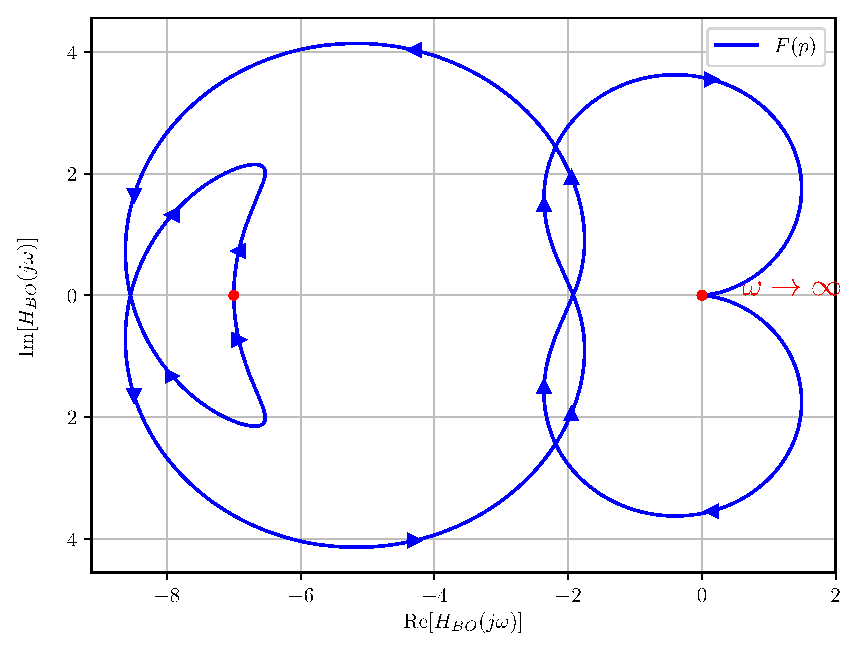
\includegraphics
    [width=0.8\textwidth]{fig/exercice_nyquist_chap_stab_ex1_enonce.eps}};
    \node at (-2,0) {\large\textcolor{col3}{$\boldsymbol{N=2}$}};
    \pgfmathsetmacro{\vx}{0.9563}
    \pgfmathsetmacro{\vy}{0.2923}
    \pgfmathsetmacro{\rr}{1.2}
    \pgfmathsetmacro{\a}{-3.75}
    \pgfmathsetmacro{\b}{1.0}
    \draw[ultra thick,col3] (\a,\b) --+ (\rr*\vx,\rr*\vy);
    \pgfmathsetmacro{\rr}{1.4}
    \pgfmathsetmacro{\a}{-4.1}
    \pgfmathsetmacro{\b}{0.5}
    \draw[ultra thick,col3] (\a,\b) --+ (\rr*\vx,\rr*\vy);
    \pgfmathsetmacro{\rr}{1.45}
    \pgfmathsetmacro{\a}{-4.3}
    \pgfmathsetmacro{\b}{0.0}
    \draw[ultra thick,col3] (\a,\b) --+ (\rr*\vx,\rr*\vy);
    \pgfmathsetmacro{\rr}{1.3}
    \pgfmathsetmacro{\a}{-4.2}
    \pgfmathsetmacro{\b}{-0.5}
    \draw[ultra thick,col3] (\a,\b) --+ (\rr*\vx,\rr*\vy);
    \pgfmathsetmacro{\rr}{1.01}
    \pgfmathsetmacro{\a}{-3.9}
    \pgfmathsetmacro{\b}{-1.0}
    \draw[ultra thick,col3] (\a,\b) --+ (\rr*\vx,\rr*\vy);
    \pgfmathsetmacro{\rr}{0.75}
    \pgfmathsetmacro{\a}{-3.35}
    \pgfmathsetmacro{\b}{-1.5}
    \draw[ultra thick,col3] (\a,\b) --+ (\rr*\vx,\rr*\vy);
\end{tikzpicture}
\end{center}
%-------------------------------------------------------------------------------

%%%%%%%%%%%%%%%%%%%%%%%%%%%%%%%%%%%%%%%%%%%%%%%%%%%%%%%%%%%%%%%%%%%%%%%%%%%%%%%%
\question{\textbf{Déterminer alors la condition sur $K$ pour ce système 
soit stable en boucle fermée.}}
%%%%%%%%%%%%%%%%%%%%%%%%%%%%%%%%%%%%%%%%%%%%%%%%%%%%%%%%%%%%%%%%%%%%%%%%%%%%%%%%
%-------------------------------------------------------------------------------
\begin{center}
\begin{tikzpicture}
    \node at (0,0) {
    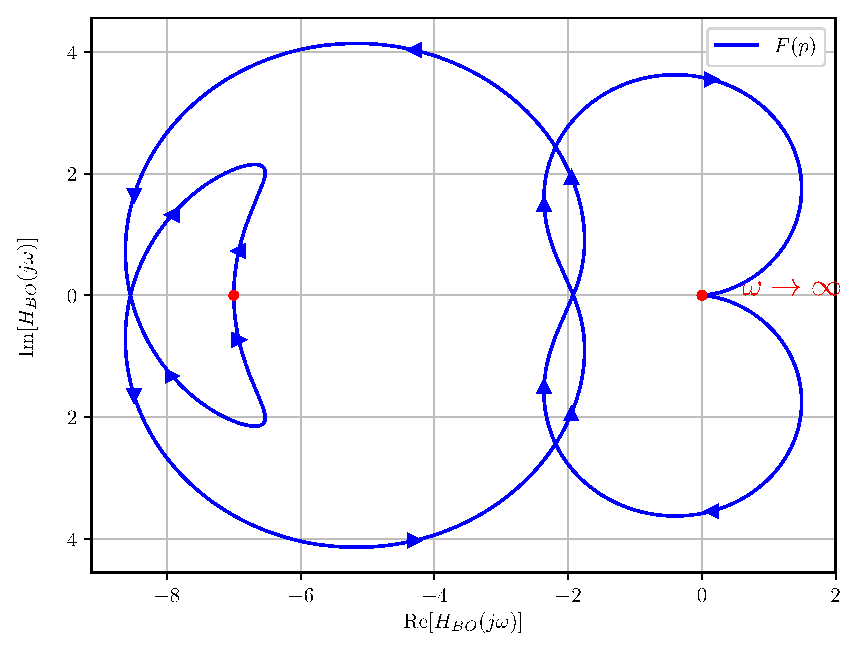
\includegraphics
    [width=0.8\textwidth]{fig/exercice_nyquist_chap_stab_ex1_enonce.eps}};
    \pgfmathsetmacro{\xu}{-4.32}
    \pgfmathsetmacro{\yu}{-0.05}
    \draw[red,fill=red] (\xu,\yu) circle (1.62pt) node[above left] {I$_1$};
    \pgfmathsetmacro{\xd}{-2.93}
    \pgfmathsetmacro{\yd}{-0.05}
    \draw[red,fill=red] (\xd,\yd) circle (1.62pt) node[above right] {I$_2$};
\end{tikzpicture}
\end{center}
%-------------------------------------------------------------------------------

Pour que le système soit stable en boucle fermée, il faut que le point 
critique de coordonnées (-1,0) se trouve entre les deux points I$_1$ et 
I$_2$ représentés sur la figure ci-dessus.
La partie réel de ces deux points est directement proportionnelle au 
gain de la boucle ouverte. Lorsque l'on augmente ou diminue le gain $K$, 
le diagramme de Nyquist est tranformé par homothétie (même forme et 
même orientation).
Ainsi, 
%-------------------------------------------------------------------------------
\begin{align*}
    K\Re{\mathrm{I}_1} < -1 \\
    K\Re{\mathrm{I}_2} > -1 
\end{align*}
%-------------------------------------------------------------------------------
%-------------------------------------------------------------------------------
\begin{align*}
    -\dfrac{1}{\Re{\mathrm{I}_2}}<K<-\dfrac{1}{\Re{\mathrm{I}_1}}
\end{align*}
%-------------------------------------------------------------------------------

On mesure sur le diagramme précédent la position des points I$_1$ et I$_2$ 
dans le cas où $K=-1$.
\begin{align*}
    \Re{\mathrm{I}_1}&=-8.544\\
    \Re{\mathrm{I}_2}&=-7
\end{align*}
donc,
\[
-0.1428<K<-0.117
\]

Nous traçons ci-dessous le diagramme de Nyquist pour $K=-0.13$
%-------------------------------------------------------------------------------
\begin{center}
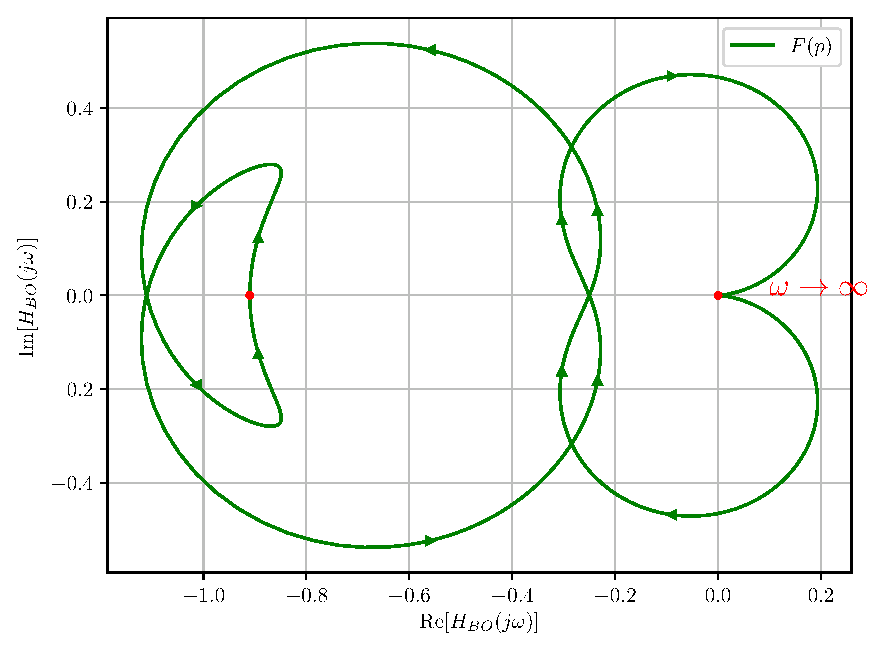
\includegraphics[width=0.8\textwidth]
{fig/exercice_nyquist_chap_stab_ex1_corrige.eps}
\end{center}
%-------------------------------------------------------------------------------


